% documentclass
% set font size=11 (11pt)
% set paper format=A4 (a4paper)
% set equation alignment to left (fleqn)
\documentclass[11pt,a4paper,fleqn]{article}


% Preamble
% to write next to images
\usepackage{graphicx,wrapfig,lipsum}
% use the inputenc and fontenc packages to use French accents
\usepackage[T1]{fontenc}
% for pseudocolor
\usepackage{algorithm,algpseudocode}
% for code samples
\usepackage{listings}
% for links
\usepackage{hyperref}
% for color
\usepackage{xcolor}
% allow for arbitrary font size
\usepackage{anyfontsize}
% set the font as Time New Roman (the Latex equivalent, at least)
% \usepackage{mathptmx}
% set the size of the document margins using the geometry package
\usepackage[lmargin=0.97in,rmargin=0.97in,tmargin=1.4in,bmargin=1.4in]{geometry}
% turn the color of footnote markers to black
\renewcommand\thefootnote{\textcolor{black}{\arabic{footnote}}}
% suppress indents on footnotes
\usepackage[hang,flushmargin]{footmisc}
% automatically generates colored brackets around references
\usepackage{fncylab} \labelformat{equation}{(#1)}
% for the bibliography
\usepackage{biblatex}
% supress indent on new paragraphs
\setlength{\parindent}{0pt}
% use the amsmath package to include mathematical symbols
\usepackage{amsmath}
% suppress the space between the left margin and the equations (fleqn still leaves some space by default)
\setlength{\mathindent}{0pt}
% create a new environment to left flush the equation with the align environment
\makeatletter
\newenvironment{lflalign}{ \vspace{-3mm}%
  \def\align@preamble{%
    &\strut@
    \setboxz@h{\@lign$\m@th\displaystyle{####}$}%
    \ifmeasuring@\savefieldlength@\fi
    \set@field
    \hfil
    \tabskip\z@skip
    &\setboxz@h{\@lign$\m@th\displaystyle{{}####}$}%
    \ifmeasuring@\savefieldlength@\fi
    \set@field
    \hfil
    \tabskip\alignsep@
  }
  \flalign}
{\endflalign}
\makeatother
% use the ammssymb package to use mathematical symbols
\usepackage{amssymb}
% remove "figure" in caption
\usepackage[labelformat=empty]{caption}
% create new commands for mathematical symbols
\DeclareMathOperator{\N}{\mathbb{N}}
\DeclareMathOperator{\Z}{\mathbb{Z}}
\DeclareMathOperator{\Q}{\mathbb{Q}}
\DeclareMathOperator{\R}{\mathbb{R}}
\DeclareMathOperator{\Pb}{\mathbb{P}}
% declare the cmsy (computer modern symbol) math alphabet to define appropriate fonts for the U and N mathematical symbols
\DeclareMathAlphabet\mathbcal{OMS}{cmsy}{m}{n}
% create new commands for mathematical symbols
\DeclareMathOperator{\E}{\mathbcal{E}}
\DeclareMathOperator{\Ex}{\mathbb{E}}
\DeclareMathOperator{\F}{\mathbcal{F}}
\DeclareMathOperator{\G}{\mathbcal{G}}
\DeclareMathOperator{\M}{\mathbcal{M}}
\DeclareMathOperator{\HH}{\mathbcal{H}}
\DeclareMathOperator{\QQ}{\mathbcal{Q}}
\DeclareMathOperator{\PP}{\mathbcal{P}}
\DeclareMathOperator{\Noo}{\mathbcal{N}}
\DeclareMathOperator{\U}{\mathbcal{U}}
% use the bbm package to be able to use the double stroke 1 for the indicator function
\usepackage{bbm}
\DeclareMathOperator{\ind}{\mathbbmss{1}}
% use the bm package to use bold characters in math mode
\usepackage{bm}
% create a new command for black square bullets
\newcommand{\bs}{\scalebox{0.7}{$\blacksquare$} \hspace{2mm}}
% use the relsize package to be abe to change the size of mathematical symbols
\usepackage{relsize}
% define a new command for in-line small summation
\newcommand{\ssumm}[2]{\underset{\scriptscriptstyle #1}{\overset{\scriptscriptstyle #2}{\mathlarger{\mathlarger{\mathlarger{\Sigma}}}}} \hspace{0.5mm}}
% define a new command for in-line small products
\newcommand{\sprod}[2]{\underset{\scriptscriptstyle #1}{\overset{\scriptscriptstyle #2}{\mathlarger{\mathlarger{\mathlarger{\Pi}}}}} \hspace{0.5mm}}
% Use the caption package to customize captions (titles) of tables and graphs
\usepackage[font=small,labelfont=bf]{caption}
% use float package to force figure the be positioned where indicated
\usepackage{float}
% use the graphicx package to be able to resize tables
\usepackage{graphicx}

\usepackage{lipsum}% Used for dummy text.
\definecolor{titlepagecolor}{cmyk}{1,.60,0,.40}
\definecolor{namecolor}{cmyk}{1,.50,0,.10} 

\begin{document}

{\fontsize{25pt}{40pt} \textbf{Clustering in Wealth Management:}\par}
{\fontsize{25pt}{40pt} \textbf{an Original Way to Visualize Client Behaviors}\par}

\section{Intro}

Wealth management consists in managing investments on behalf of others. To provide the best service, it's crucial for wealth managers to understand clients' behaviors. That's why it's common in private banks to look for patterns within clients' data. Clustering is a common method to achieve this. However, one of the key challenge with such approach is to display and interpret the results. In this article I will briefly give an introduction to clustering and most of all, show a simple and original way to display the results. Below is an insight of the final results.

\begin{center}
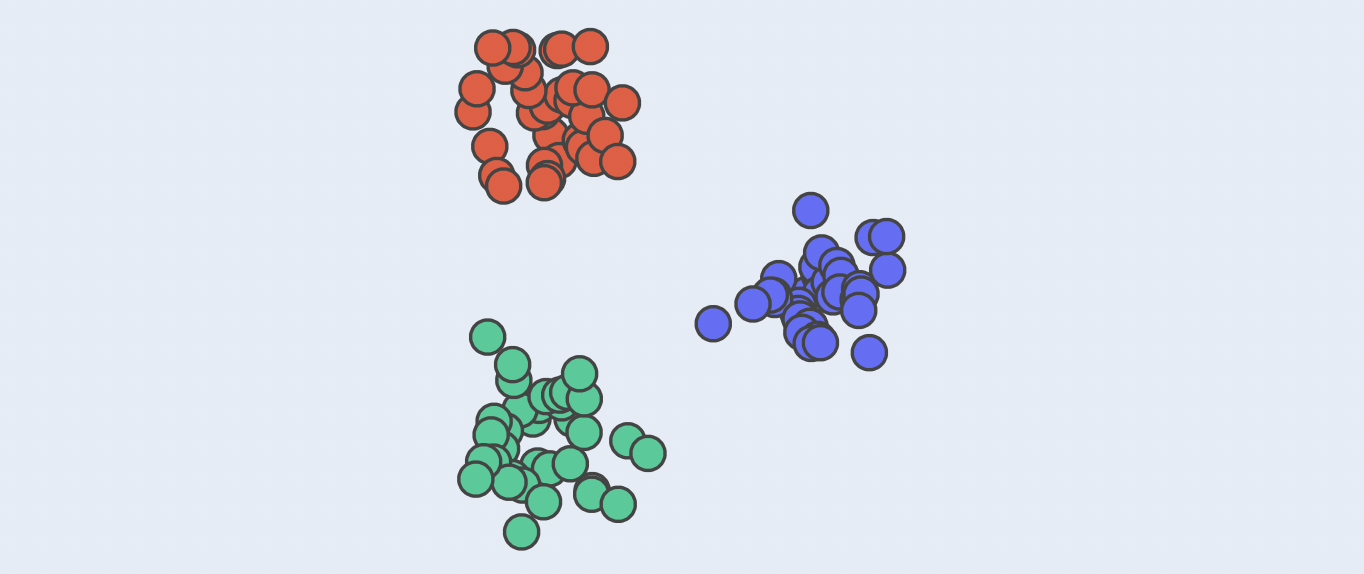
\includegraphics[scale=0.5]{./../img/clusters-static.png}
\end{center}

\section{Example}

We use a toy example to make the method easier to understand. Say we have a bank with 10 clients. We want to focus on the main characteristics of those clients. In this example we consider only 4 aspects (as you can imagine, this is very simplified): \\

- Wealth (also called asset under management) \\
- Number of unique financial instruments \\
- Number of transactions \\
- Age

\section{Clustering}

Clustering is about grouping clients based on similar characteristics. There are numerous ways of performing such tasks and discussing those different methods is not in the scope of this article. Let's use a common clustering method, the \href{https://en.wikipedia.org/wiki/Mixture_model}{Gaussian Mixture}. In a nutshell, this method allows to estimate the density of each cluster. For more mathematical details, check out my notes \href{https://savoga.github.io/machinelearning/gmm/}{here}.

\section{Validation}

The tricky part of any clustering method is to make sure the clusters are of good quality i.e. compact enough. We call this process the validation step. Validating our results is not the main topic of this article but I need to dig in few notions so that the visualization part will be clear. \\
In order to validate our model, we need to find a metric that represents the cluster quality to be optimized.
The chosen quality metric is the \href{https://en.wikipedia.org/wiki/Silhouette_(clustering)}{silhouette coefficient} i.e. the ratio of the distance intra/inter clusters. It measures how compact is the cluster. 

$$s(i) = \frac{b(i)-a(i)}{max(a(i),b(i))}$$

Where: \\
$a(i)$ = average distance of client i with the other points from the same cluster. \\
$b(i)$ = average distance of i with the other points from the closest cluster. \\

The below picture helps to understand better what those distances mean exactly. 

\begin{center}
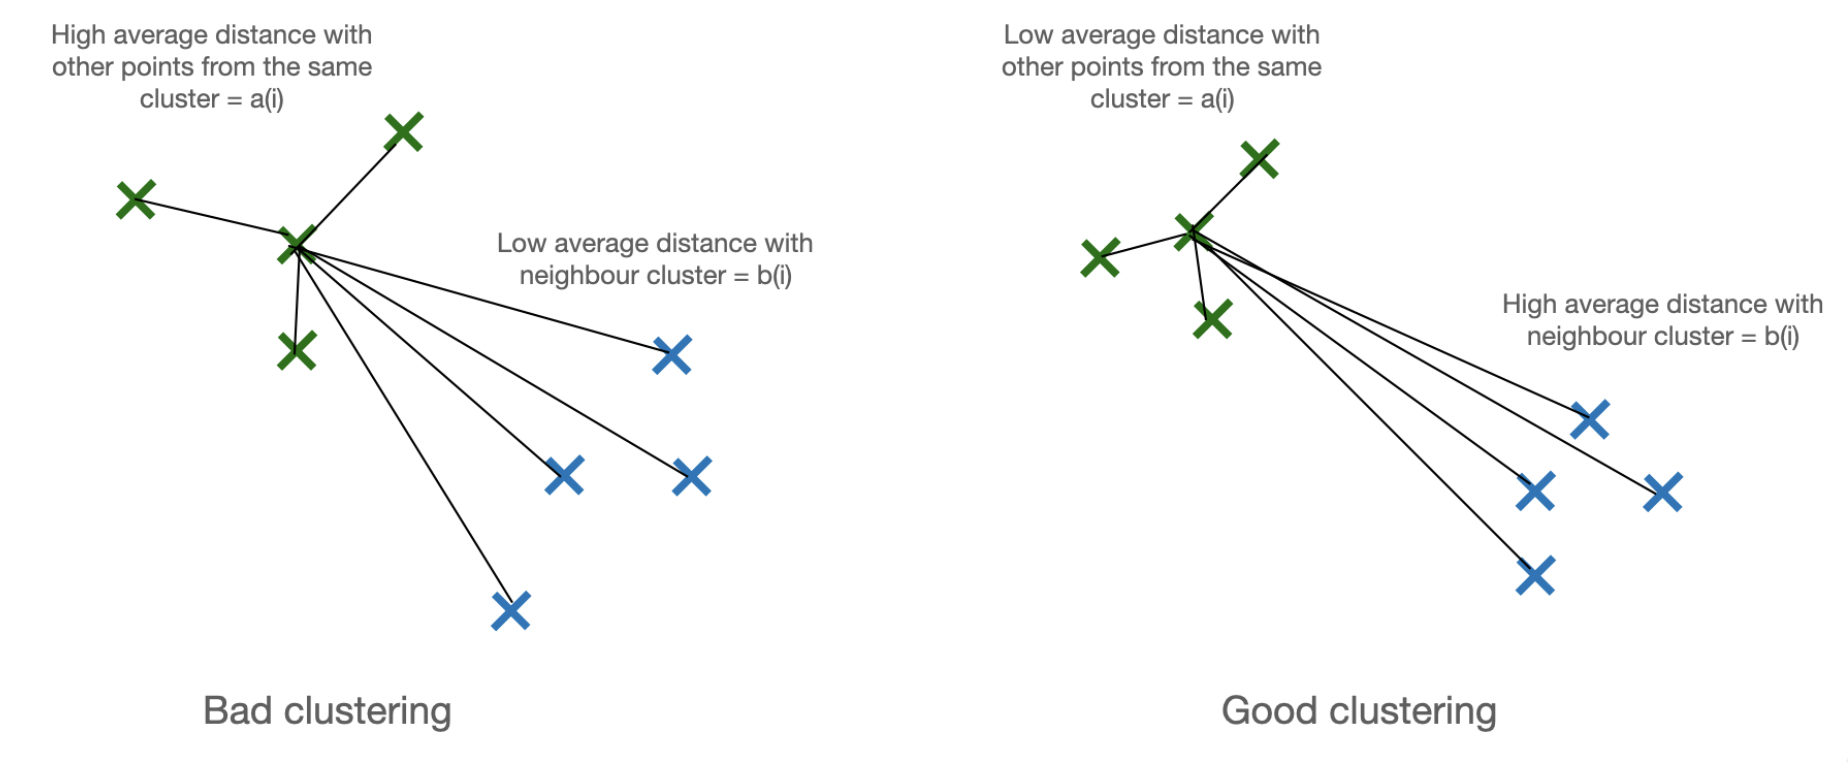
\includegraphics[scale=0.5]{./../img/silhouette-explanations.png}
\end{center}

The higher the silhouette coefficient, the better is the cluster quality. We can thus test different parameters and chose the combination that gives us the best silhouette coefficient. \\

\textit{Note: the silhouette coefficient is NOT adapted if you use a clustering method that can identify non convex clusters. For more information, I recommend the \href{https://scikit-learn.org/stable/modules/clustering.html}{scikit learn's user guide}.}


\section{Visualization}

Now that our clusters are well defined, how do we visualize the results? More specifically, how to communicate our results to the rest of our colleagues in a meaningful way?
When researching on the topic on how to best perform cluster visualization, I came across many methods that involve \href{https://en.wikipedia.org/wiki/Dimensionality_reduction}{dimension reduction}. In short, it consists in transforming our problem to a 2D case. That way we could display results that humans are capable of reading graphically. The problem with this transformation is that we \textbf{lose important aspects of the data (variability)}.
One way to overcome this problem is to display only the density. After all, when performing a clustering task the key questions are:

- How precise are the detected patterns? \\
- How good an observation (i.e. a client) "fit" into a specific cluster? \\

Displaying the density allows to answer those questions. We will build a solution based on the silhouette coefficient described above. \\

\underline{Step 1: define centers for each cluster} \\

First, we define the center coordinates for each cluster. We want to make sure each cluster is distinct so that it's readable enough. To do so, we find the coordinates of the points that are located on a circle (radius 1) and are equidistant. If we would end up with 10 clusters, the centers would be separated as such:

\begin{center}
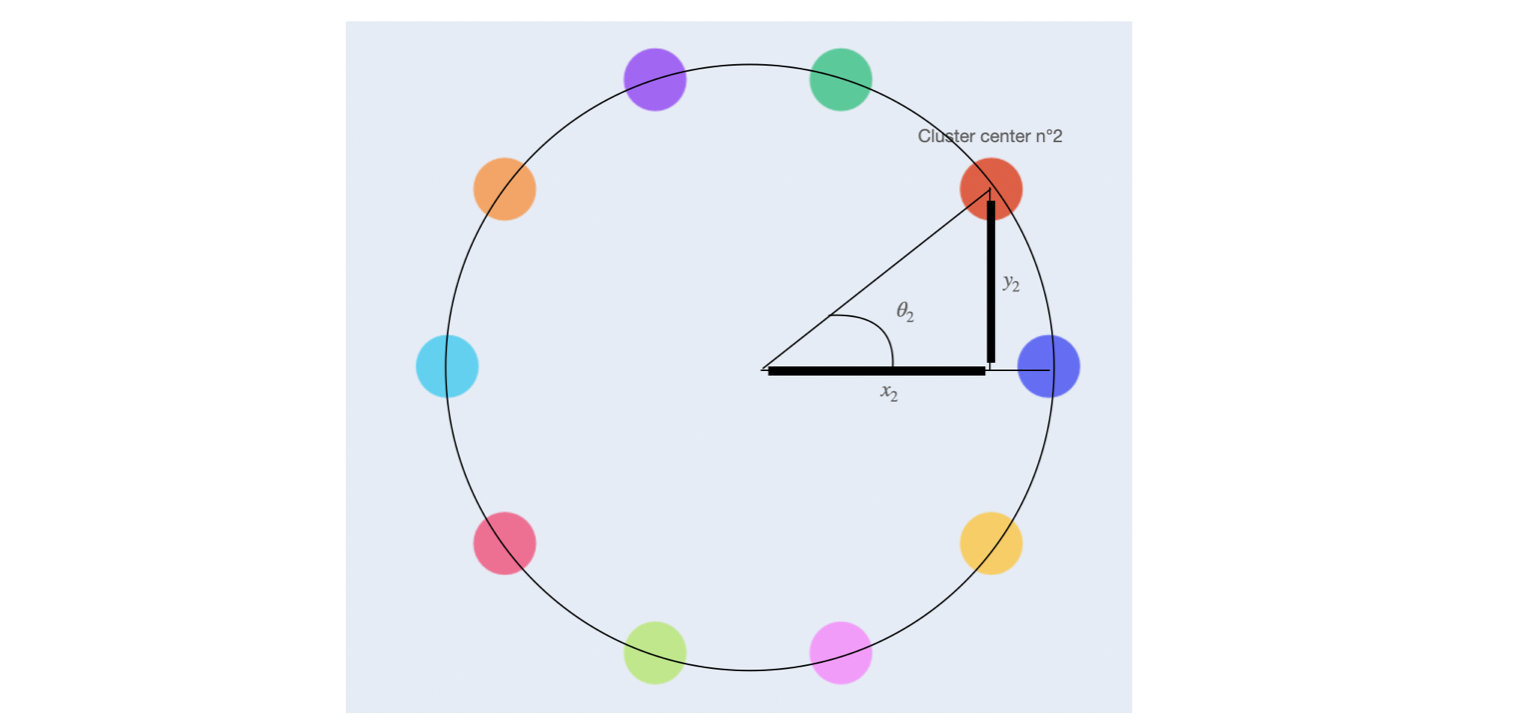
\includegraphics[scale=0.5]{./../img/10-clusters-angle-3}
\end{center}

The coordinates are found using the cosinus/sinus of thetas that correspond to the equidistant points on the circle. The full details can be found in the \href{https://github.com/savoga/clustering-visualization-article/blob/main/clustering-visualization-article.ipynb}{code}. \\

\underline{Step 2: generate coordinates for each cluster} \\

Each cluster's observations are generated with a normal distribution where the center is the center of the cluster from the previous step and the standard deviation is the quality of the cluster. 
For each cluster, we find the coordinates x and y:

$$x \sim \mathcal{N}(\mu_x, 1-silhouette)$$

$$y \sim \mathcal{N}(\mu_y, 1-silhouette)$$

where $\mu_x$ is the first coordinate of the cluster center found in the previous step. The silhouette is the coefficient corresponding to the quality of the cluster. \\

You may ask yourself: why do we generate data? and why do we use the silhouette as standard deviation? We generate data since we focus on density (as explained above), that is, how close are observations with each other. The standard deviation represents the compactness of our clusters - the higher the standard deviation, the less compact are the clusters. We can thus use the opposite of the silhouette coefficient. \\

\underline{Step 3: compute the distance to center} \\

We compute the distance of each generated point to the center of the cluster. A simple Euclidean distance would work fine. \\

\underline{Step 4: map each point to the right generated point} \\

Finally, we sort the data based on their distance to the center. We map observations so that, for each observation, the distance to the cluster center is proportional to silhouette coefficient. That way, we penalize observations that seem to fit poorly to the cluster they belong to (based on the silhouette coefficient).

\section{Results}

From the below figure, we can see that two clients are more distant from their cluster centers. This means that their profile is not fitting as good as other peers from the same cluster. Indeed, the first client on the left (green) has a much lower wealth than others. However, his trading behavior makes him a good candidate for this cluster. Similarly, the client on the right (blue) has a slightly larger number of trades than others from the same cluster. The full data can be found in this \href{https://github.com/savoga/clustering-visualization-article/blob/main/clustering-visualization-article.ipynb}{notebook}.

\begin{center}
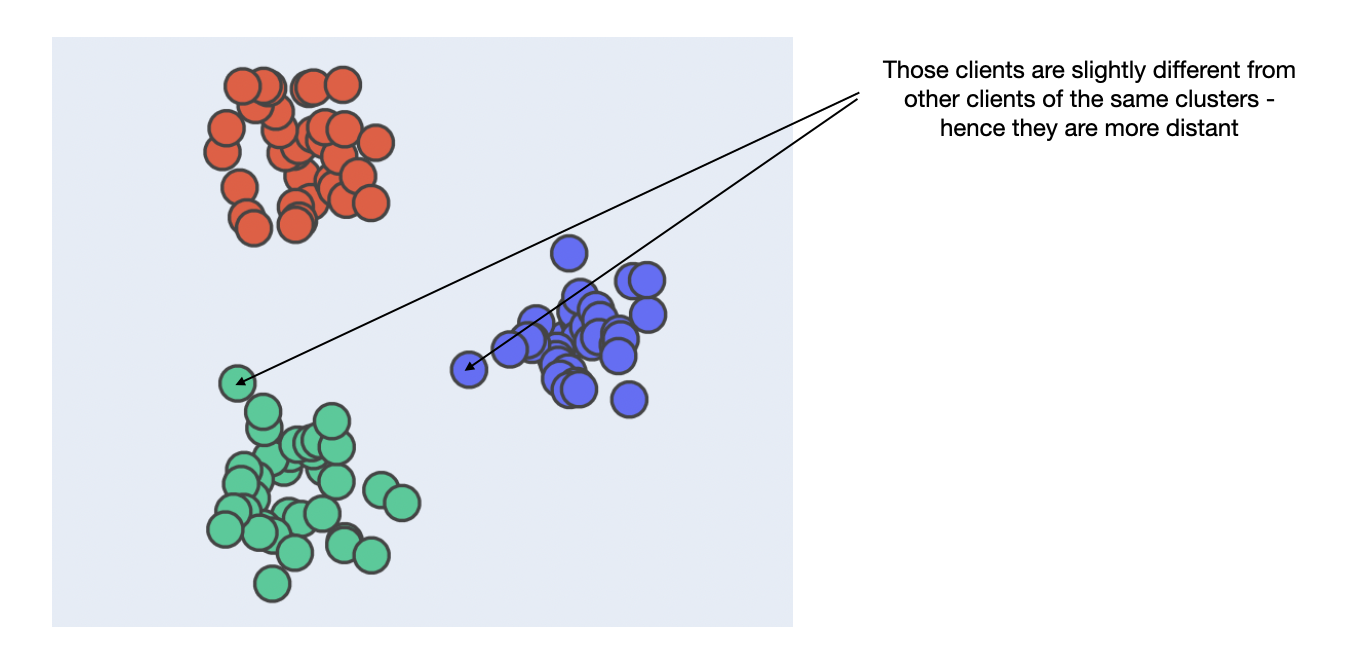
\includegraphics[scale=0.5]{./../img/clusters-static-arrow.png}
\end{center}

\textit{Note}: from this figure, we can draw conclusions only from the dots and their respective cluster centers. The distances between dots other than the center is not relevant, as well as the distances between clusters. This could represent a potential development of the method. \\

\textit{Note (2)}: the graphical library that I use is \href{https://plotly.com/}{Plotly}. It's a well maintained and highly customizable package that I highly recommend.

\section{Conclusion}

In this article, I have presented a method to display cluster results focusing on the density. Using such method, wealth managers can quickly see whether there are large/small groups of clients behaving similarly, identify clients with strong profiles as well as potential outliers.

\section{References}

Clustering GMM (1) - https://en.wikipedia.org/wiki/Mixture\_model \\

Clustering GMM (2)  - the following blog gives quite a good explanation of the concept: https://jaketae.github.io/study/gaussian-mixture-models/ \\

Silhouette coefficient - https://en.wikipedia.org/wiki/Silhouette\_(clustering) \\

Plotly - https://plotly.com/ \\


\vspace{10mm}

\end{document} 